\section{Context}
\label{design:context}

During the bootstrapping process, the bootware has to know certain things to be able do its job.
For example, it has to know which plugins it should use to process a request or which login credentials it should use to authenticate itself with a cloud provider.
This information can be combined in one central object, which defines the nature of the current request: The context.
The bootware will read the information provided in the context at various stages of the bootstrapping process to load plugins or to supply them with a particular configuration set required for a request.
In this section we will take a closer look at this context object and its content.
How exactly the context is implemented is shown in \autoref{implementation:context}.

\begin{figure}[!htbp]
	\centering
	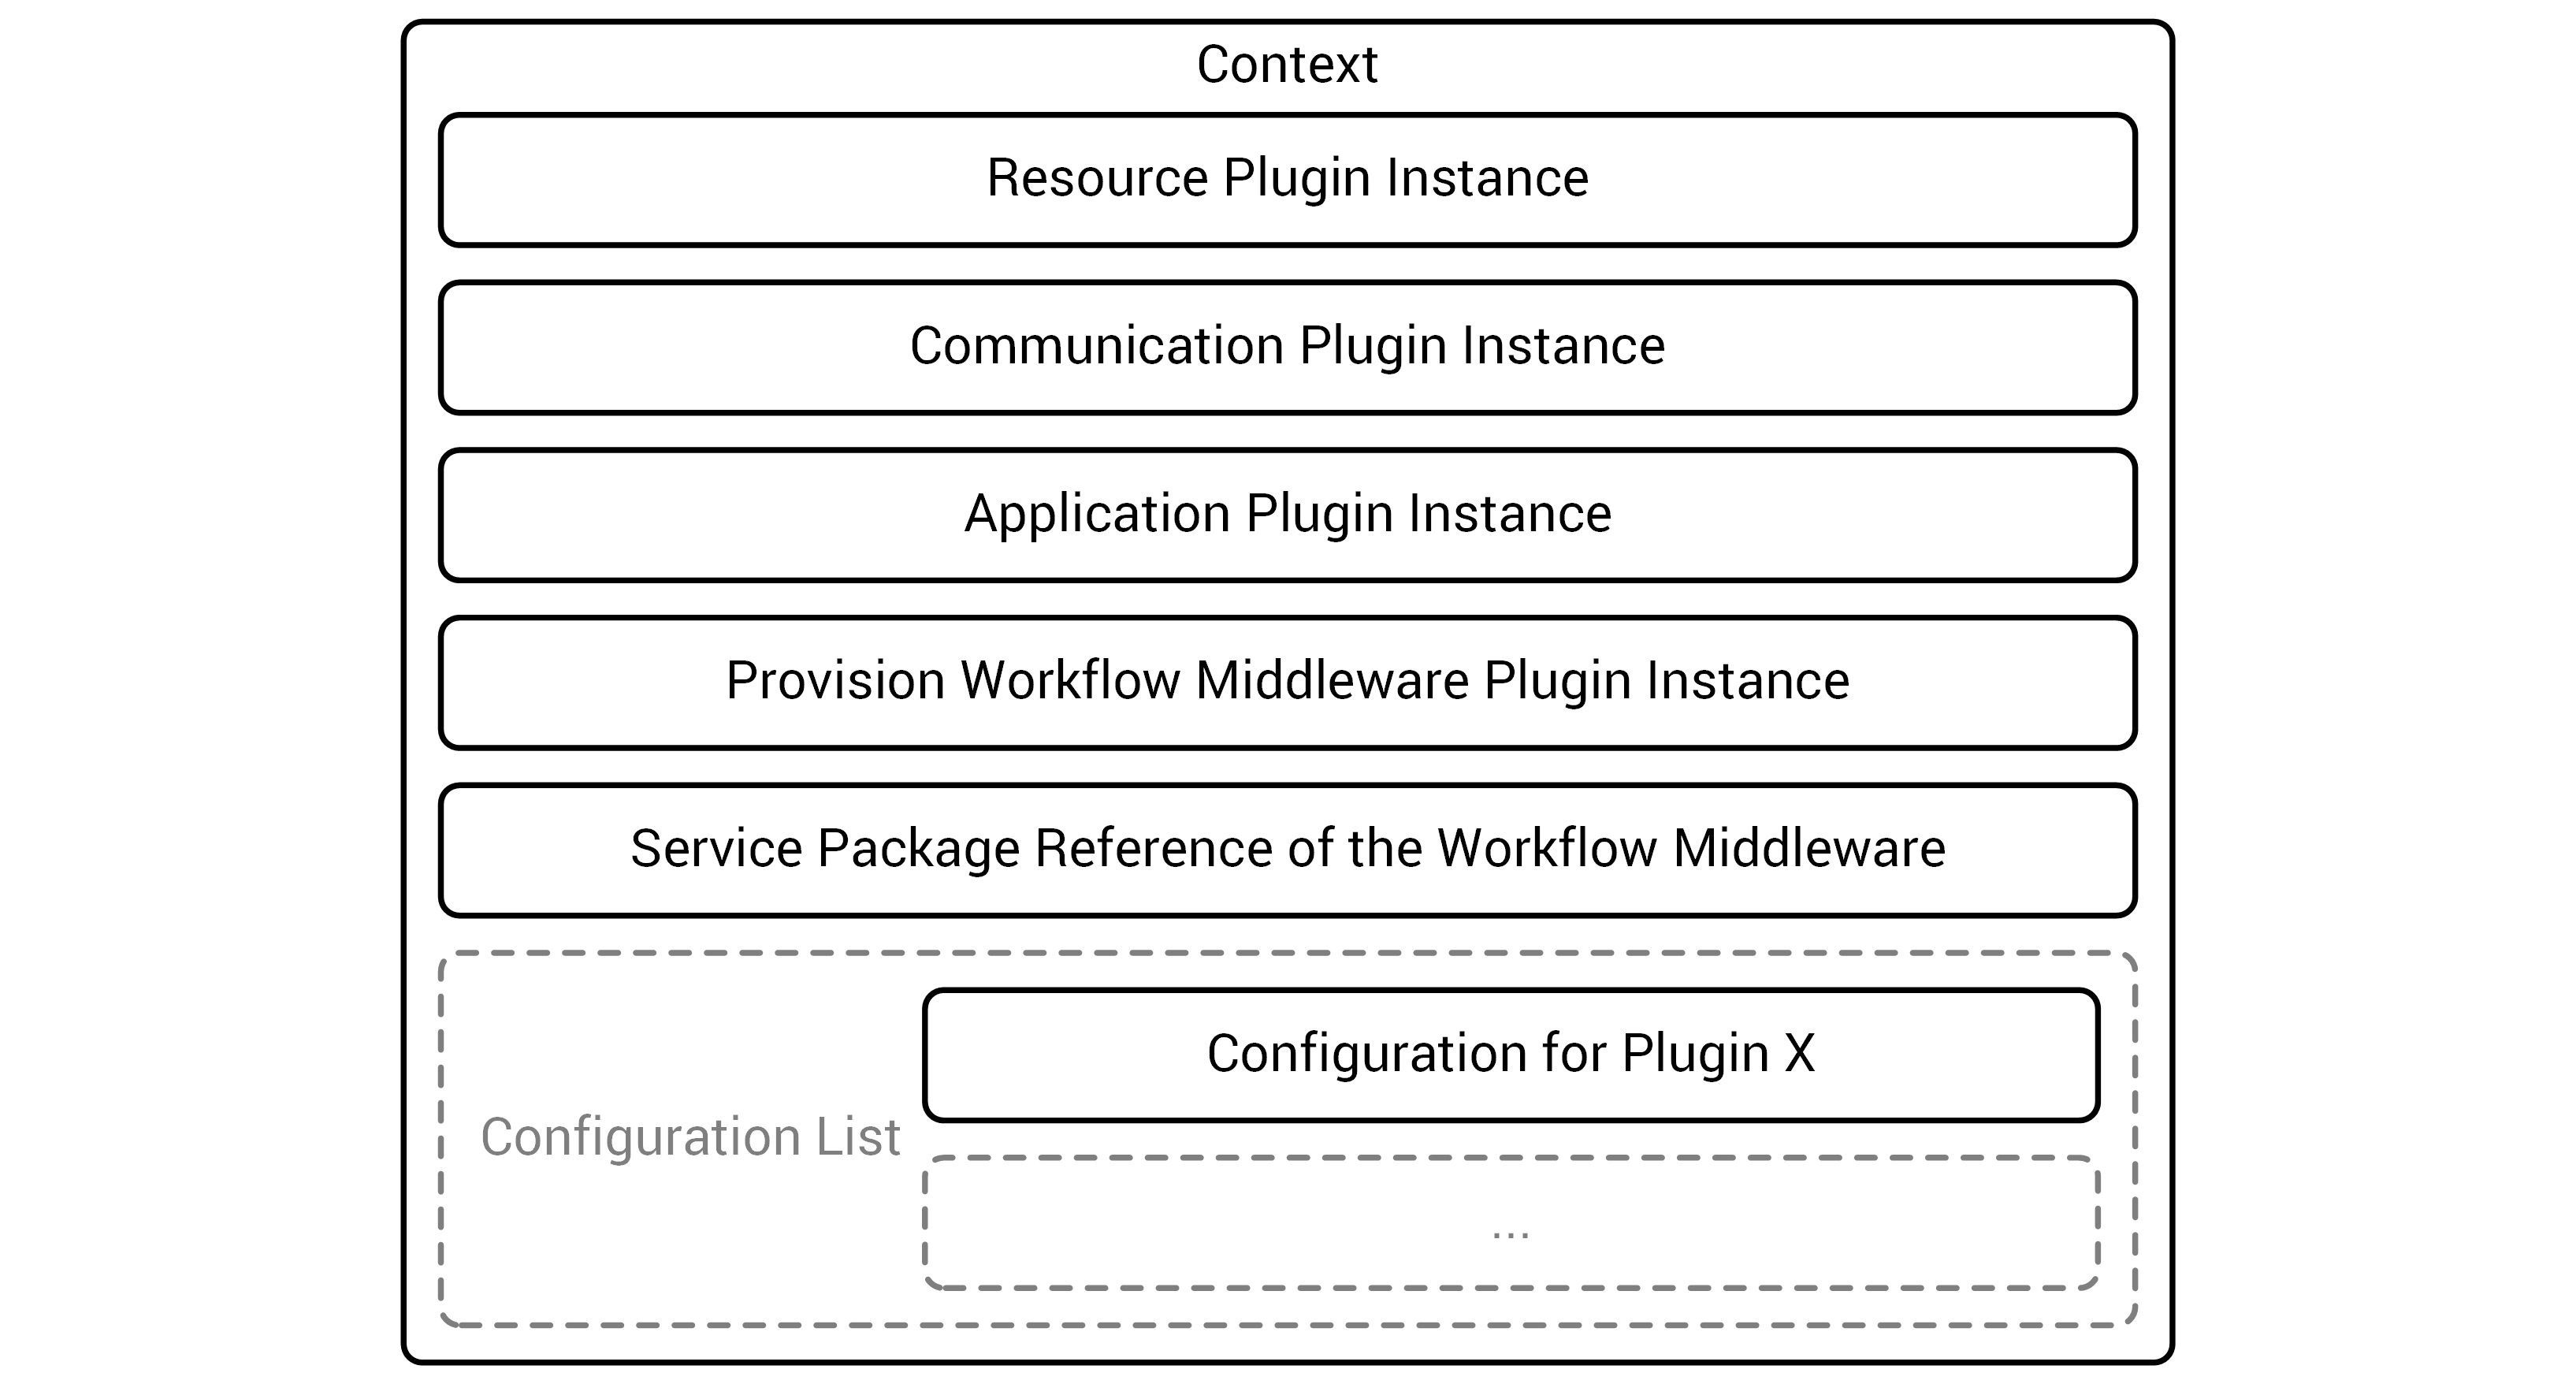
\includegraphics[resolution=600]{design/assets/context}
	\caption{Content of the context object.}
	\label{image:context}
\end{figure}

\autoref{image:context} shows the context object and its content.
As we can see in the upper half, it defines the plugin instances to be used for the current request.
The resource plugin instance defines, which resource plugin should be used to provision the requested resource.
The communication plugin instance selects, which communication plugin the bootware should use to connect to this resource.
The application plugin instance defines the application that should be provisioned on this resource, which will be a provisioning engine in our case.
Finally, the provision workflow middleware plugin instance defines the plugin that should be used to call this provisioning engine to provision the workflow middleware.
It will use the service package reference of the workflow middleware, which is also defined in the context, as input to start the provisioning of the workflow middleware.

In the bottom half of \autoref{image:context} we can see that the context can also contain configuration for different plugins.
This is necessary because various plugins might need to be configured properly to be able to fulfill their task.
For example, most resource plugins will need some kind of login credentials to authenticate with the resource provider.
As another example, when creating a EC2 instance in the Amazon cloud, the user also has to select in which region this instance should be created and which ports should be opened.
These and other configuration details can be supplied from the outside with the context.
In the future, the context might be extended to hold additional information, but for this diploma thesis, this context will be sufficient.

This context has to somehow be generated from the information the bootware receives with each request.
However, components outside of the bootware should not know anything about the inner workings of the bootware, i.e. which plugins are used to fulfill a request.
All information that might be supplied with a request can be seen in \autoref{image:request_context}.
The resource parameter specifies, which resource should be used (e.g. a specific cloud provider).
The application parameter specifies the application that should be deployed on this resource (e.g. a specific provisioning engine).
The service package reference of the workflow middleware is used by the bootware to retrieve the service package to provision the workflow middleware.
In the configuration list, configuration values that have to be supplied from the outside can be specified, such as login credentials for a cloud provider.

\begin{figure}[!htbp]
	\centering
	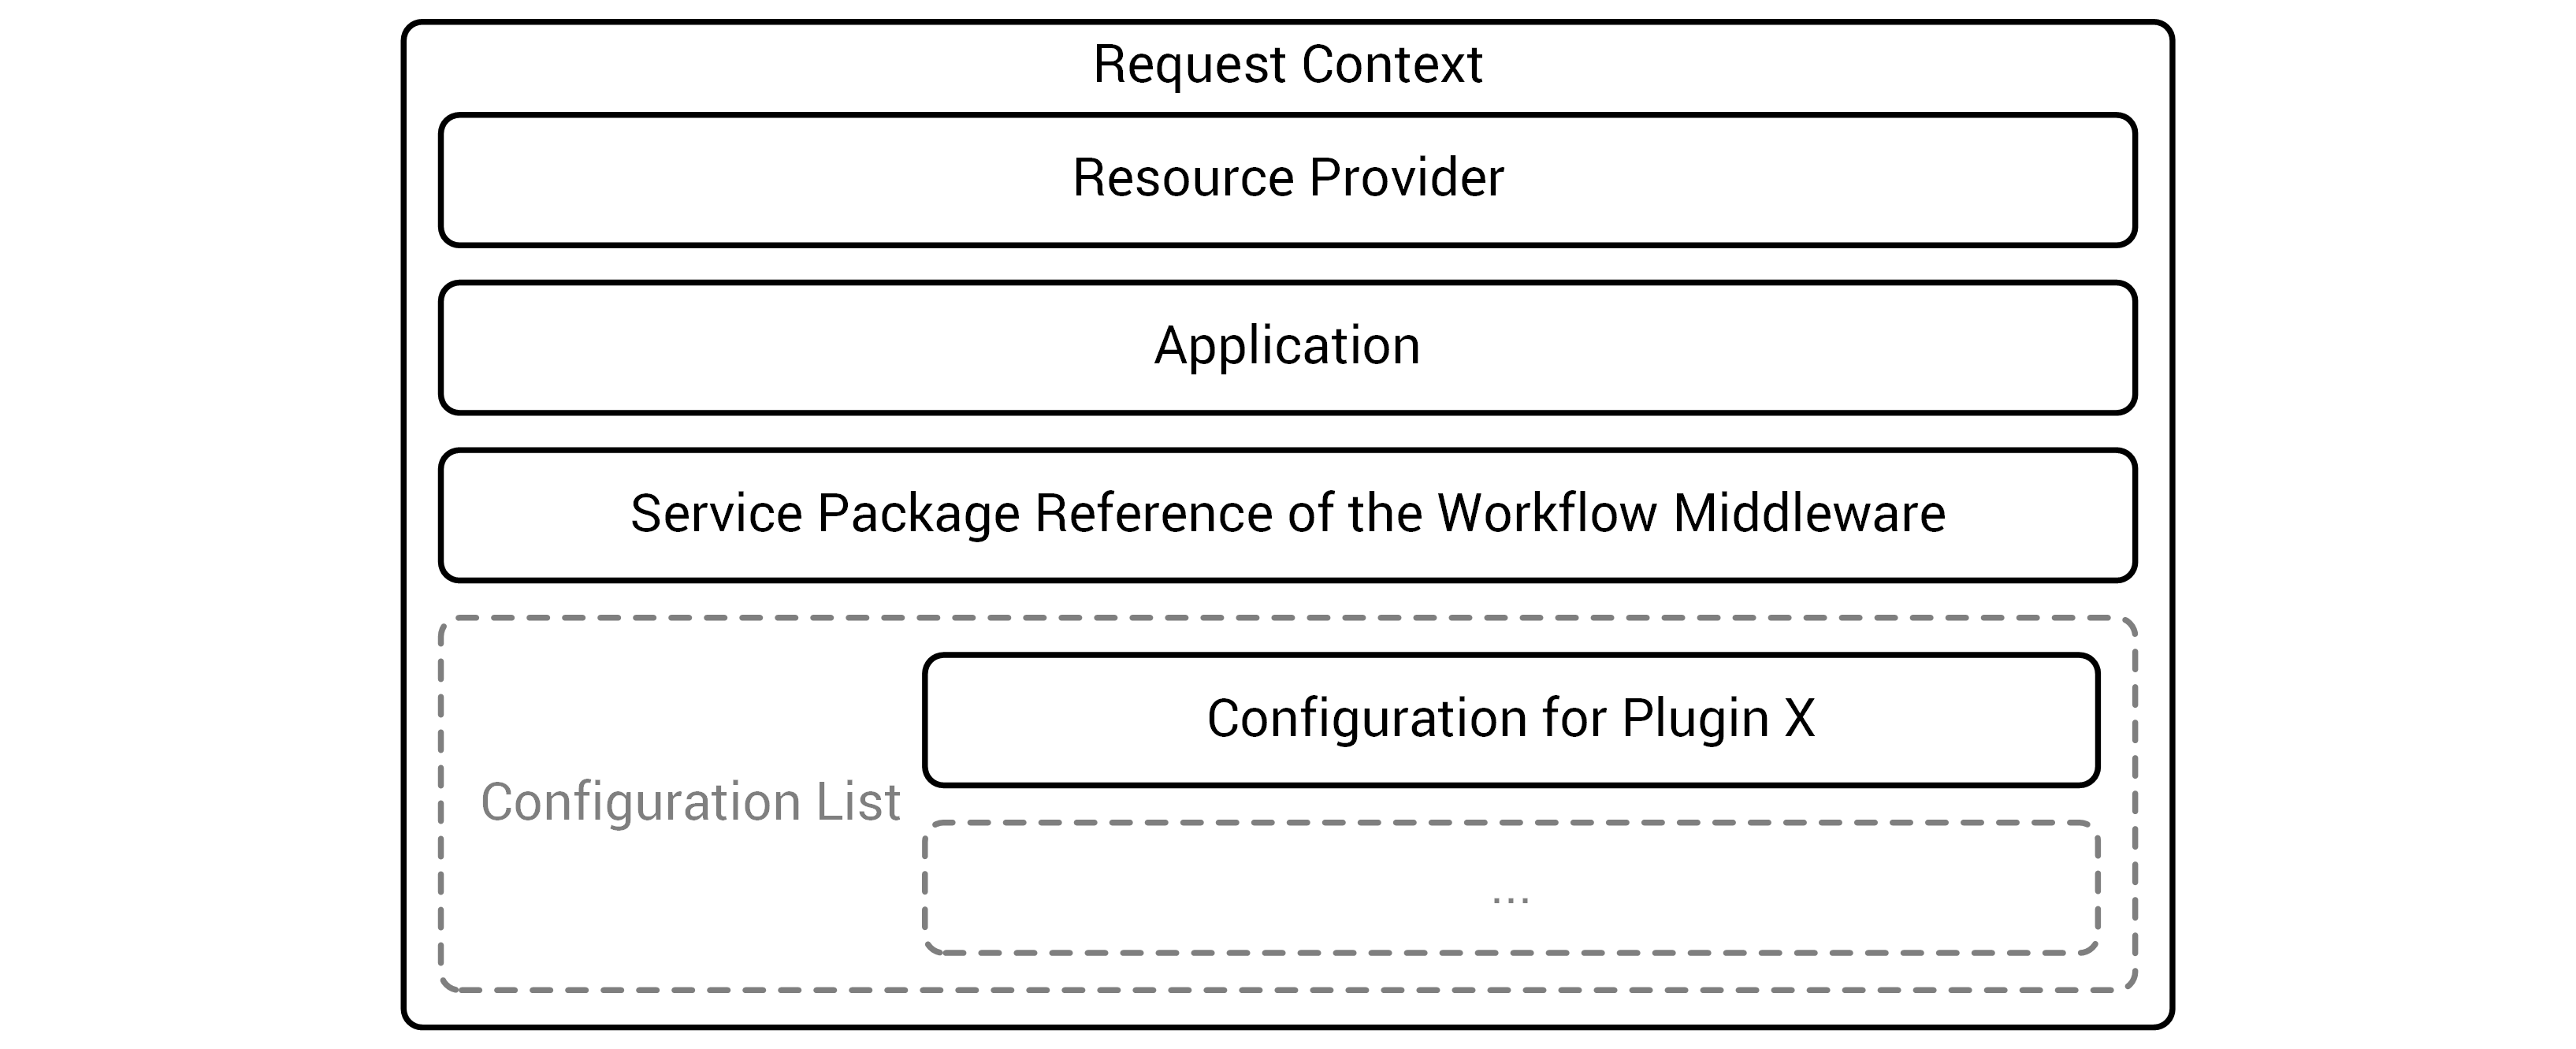
\includegraphics[resolution=600]{design/assets/request_context}
	\caption{Information send with a request.}
	\label{image:request_context}
\end{figure}

Based on this information the bootware has to decide which specific plugin instances should be used to process the request.
In the future, this could be done by querying a registry with this information, which would then return a set of specific plugins and settings.
\autoref{image:mapping} shows an exemplary mapping of the parameters supplied in a request to the specific plugins instances and configuration.
In this example, the request wants OpenTOSCA in an Amazon cloud.
The registry would then look up, if a registry entry exists for this set of parameters.
In this case, the registry contains applications as primary keys and resources as secondary keys.
The entry returned for a specific parameter combination contains the specific plugin instances and additional configuration parameters that are necessary to provision the requested application on the requested resource.

\begin{figure}[!htbp]
	\centering
	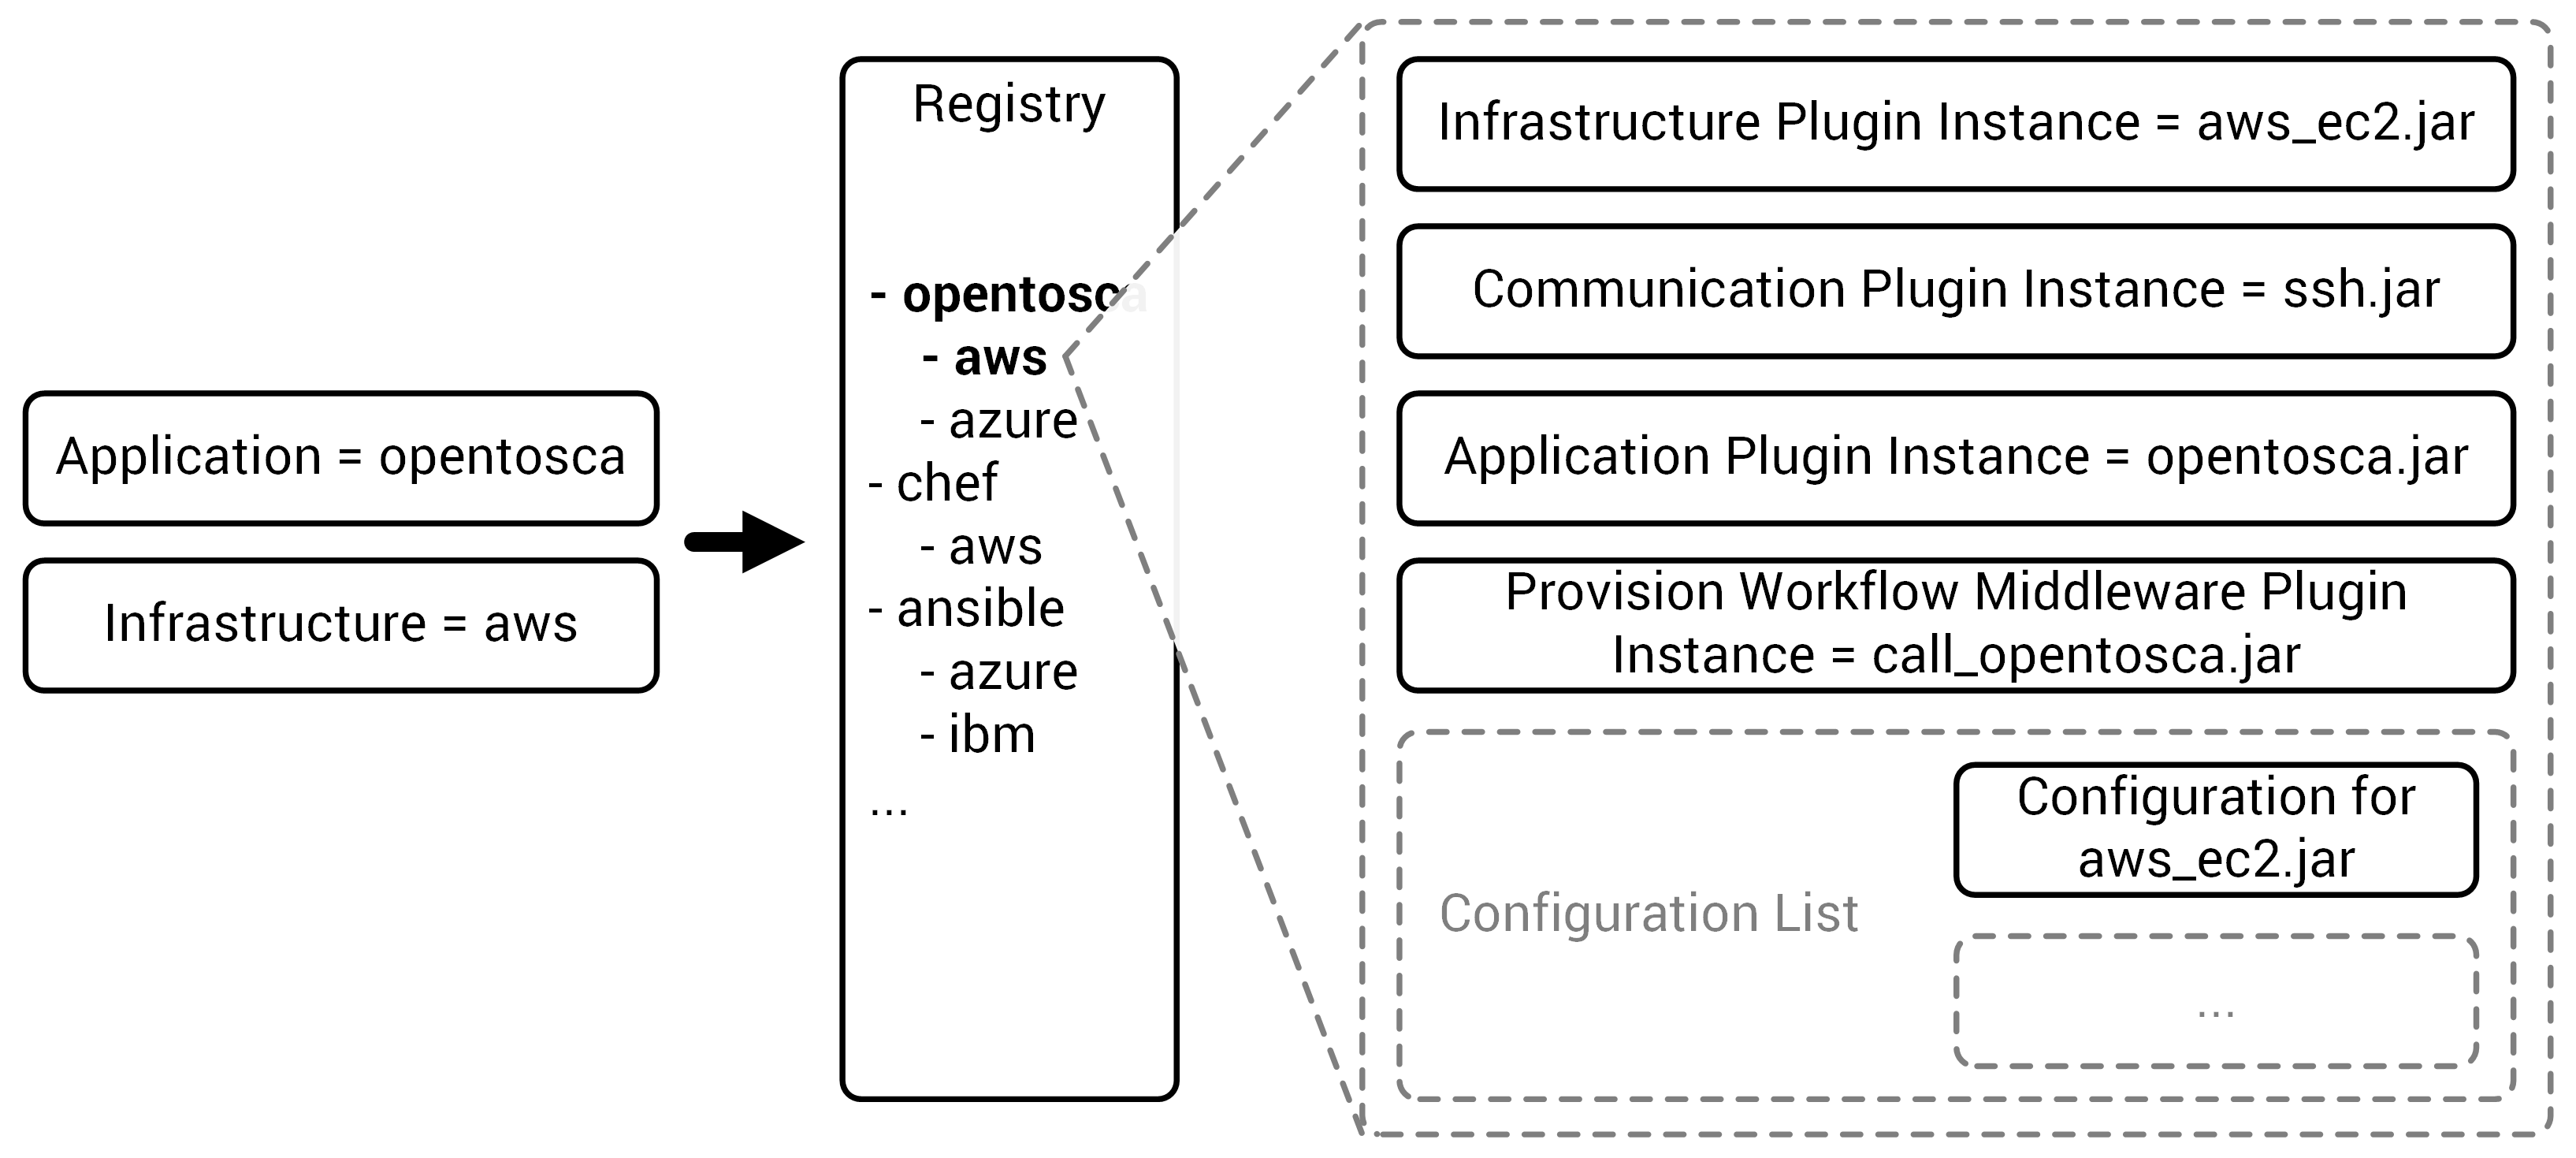
\includegraphics[resolution=600]{design/assets/mapping}
	\caption{Mapping of the request parameters to specific plugins.}
	\label{image:mapping}
\end{figure}

The bootware has to combine the information received in a request with the information that it received from the registry by merging the two sets into the final context.
However, there is one caveat in this scenario.
Right now, other components making a request to the bootware would have to supply configuration parameters like login credentials with each request.
Unlike the other request parameters, the configuration might not change between requests.
Additionally, the other components calling the bootware, may not know (and maybe should not know) anything about some content of the configuration, like login credentials.
While this might change in the future, it would make sense to be able to set the configuration once when starting the bootware, so that it does not have to be delivered with each request and so that other components can still use the bootware without also sending a configuration.
It should however still be possible to override or update the configuration at a later point.
Overriding would allow any request to temporarily use other configuration values if necessary.
Updating the configuration at a later point could be useful, for example if the user accidentally provided the wrong credentials at the beginning.
Without this functionality, the whole bootware process could fail (even while provisioning the very last service) and would have to be started again from the beginning.
This could be avoided by providing the functionality to change the configuration even during the bootstrapping process.

For setting the configuration at the beginning and for updating it later during the process, a \textit{setConfiguration} method will be added to the bootware web service.
The configuration set by this method will be treated as the default configuration by the bootware.
It will be used during the process if no other configuration is provided.
If however a request is sent with a configuration that also contains values already set in the default configuration, these values will override already existing default values temporarily for this request.
This behavior could also be extended to other parts of the context in the future if necessary.

\begin{figure}[!htbp]
	\centering
	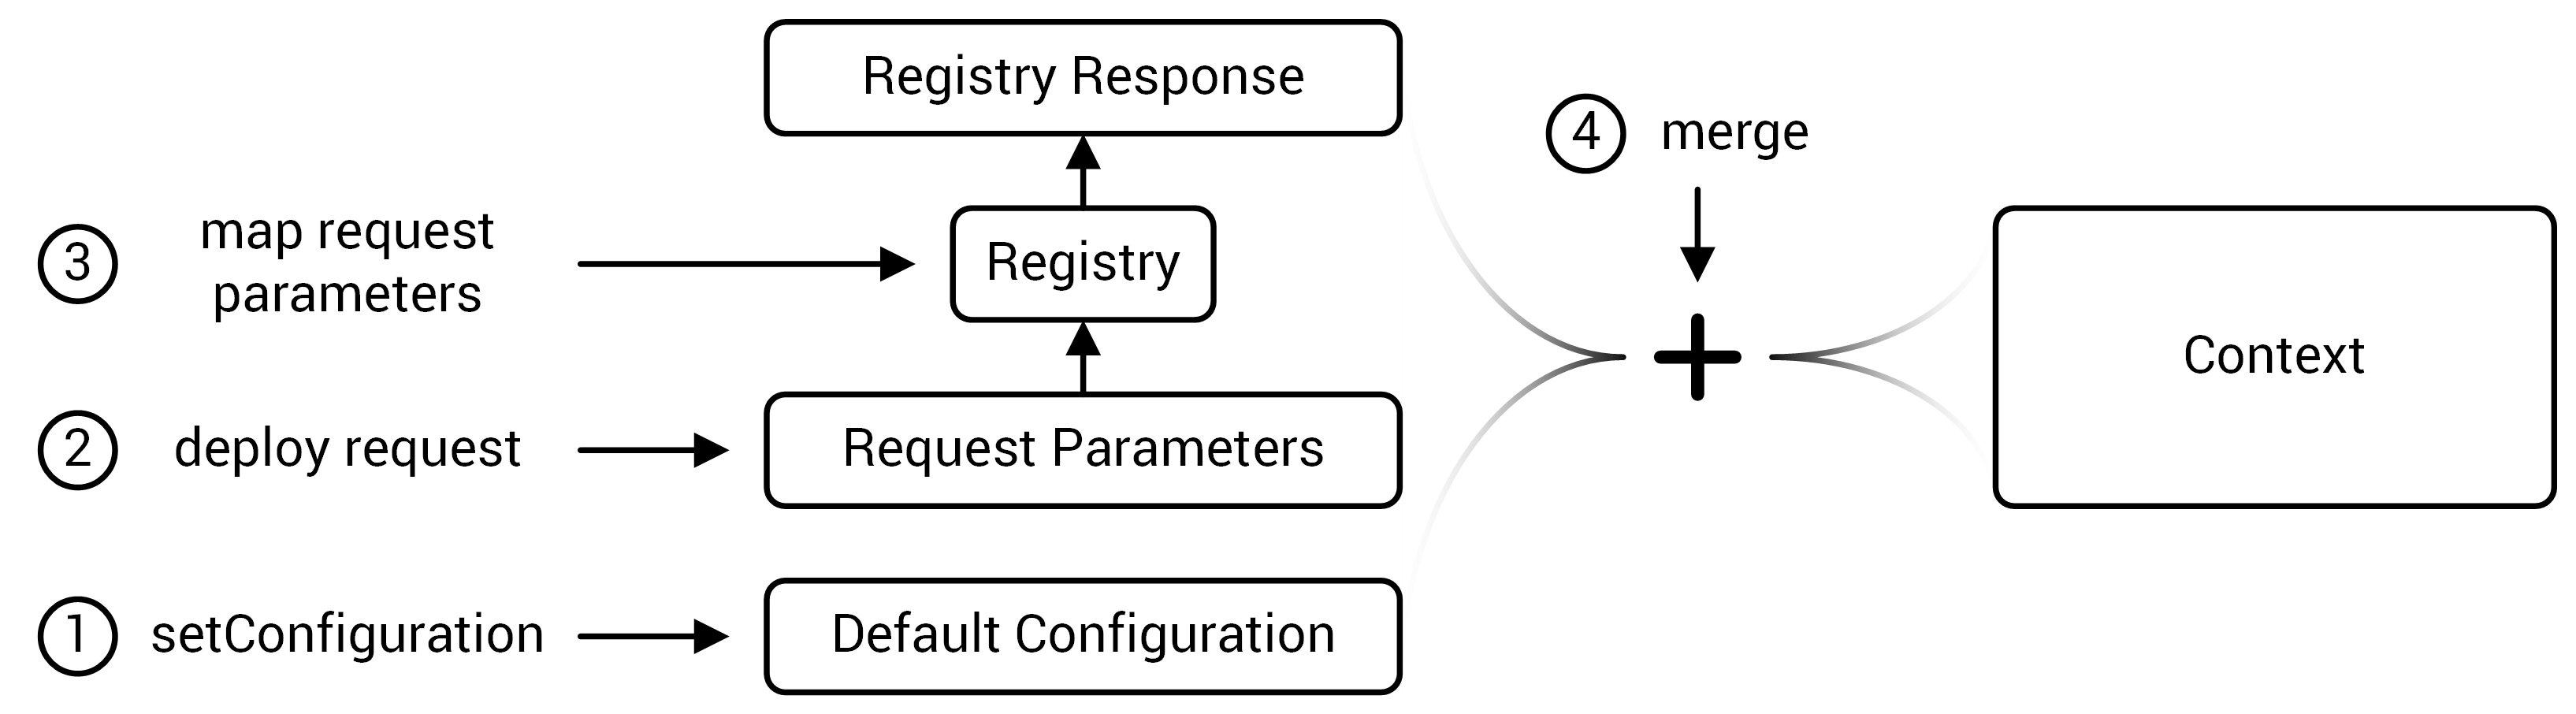
\includegraphics[resolution=600]{design/assets/merge}
	\caption{Building the final context through merging.}
	\label{image:merge}
\end{figure}

\autoref{image:merge} shows the merging process which now merges the default configuration, the request parameters, and the response from the registry.
In step one, at the beginning of the bootware execution, the default configuration is set using the \textit{setConfiguration} operation.
A deploy request is received in step two, which contains the request parameters as shown in \autoref{image:request_context}.
In step three, the request parameters are mapped to specific plugin instances and additional configuration using the registry.
In step four, the default Configuration, the request parameters, and the registry response are merged into the final context object.
This context object is then used to fulfill the request.

While we have planned to use a registry for mapping request parameters to concrete values, due to time constrains we were not able to specify this registry in more detail or implement it in our prototype.
For our implementation we use a local mechanism for mapping the request parameters.
The registry is left for future work and will not be covered further in this diploma thesis.
